\documentclass[../../main.tex]{subfiles}
\begin{document}

This section will concern the design and implementation of the functionality on the FPGA as well as the microcontroller. The microcontroller is to handle the computation of the PID-controllers, SPI communication and user-input. The FPGA is to handle the PWM signal, direction of the motors and the data from the encoders used for the position and velocity. 



\subsection{FPGA} \label{subsec:SystemImplemtationFPGA}
% \subsubsection*{Description of the Robot}

% \begin{figure}
%     \centering
%     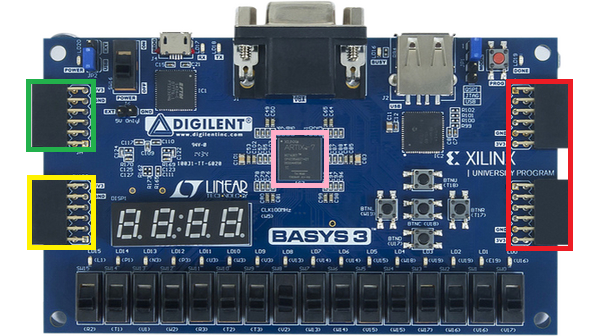
\includegraphics[width=0.6\textwidth]{Sections/System_Implementation/Images/Basys-3-kit.png}
%     \caption{Basys-3 development kit. The PMOD-connectors highlighted in red are used to interface with the robot. The PMOD-connector highlighted in green is used for interfacing with the microcontroller. The PMOD-connector highlighted in yellow is used for the in-board analog-to-digital-converter, that would have been used for the current measurement, had the current controller been implemented. The pink box highlights the FPGA-chip. All other peripherals (switches, LEDs, buttons, etch) on the board is not used in the project.}
%     \label{fig:Basys-3-kit}
% \end{figure}

% The system is implemented on a Basys-3 development kit shown in figure \ref{fig:Basys-3-kit}. The figure highlights the connectors used for interfacing with the robot and for interfacing with the micro-controller. For interfacing with the robot two PMOD-connectors are used, one dedicated to giving input to the robot and the other dedicated to receiving outputs from the robot. As described in section \ref{sec:ProblemDescription} the robot has two motors, each one requiring a H-bridge for control and each H-bridge requiring three inputs, yielding six inputs in total for the robot. 

\subsubsection*{Logic Implemented in the FPGA}

The logic implemented in the FPGA is divided into modules. Table \ref{tab:FPGAModulesDescription} gives an overview and a short description of each module and its function. Speed, Encoder, PWM and Reset logic modules are implemented twice, one for each motor. Figure \ref{fig:FPGALogicBothMotors} illustrates the logic implemented on the FPGA and the relation between the different modules.     
\begin{table}[]
    \centering
    
    \begin{tabular}{l|p{0.8\textwidth}}[] %{p{0.12\linewidth}p{0.4\textwidth}p{0.38\textwidth}}
        Module & Description \\
        \hline
        Encoder Module & Interfaces with and takes inputs from the pan-tilt system. Channel A and B of the encoders are read continuously and from this information a signed position relative to the original reference is calculated, which is the output of the module. \\
        \hline
        Speed Module & Calculates a speed related to the time period between two encoder pulses. Also provides a flag for determining when a frame is not moving.\\
        \hline
        Reset Module & Interfaces with the index signal of a frame and uses this signal to reset the frame. \\
        \hline
        Protocol Module & Used to determining which duty cycle is passed on to the PWM-module and enabling the reset routine. \\
        \hline
        SPI Module & Interfaces with the microcontroller. Contains an SPI slave for each type of information going to or from the microcontroller. \\
        \hline
        PWM Module & Interfaces with the H-bridge. Takes in a 10 bit value used to determine the duty-cycle. The frequency of the pulse-width-modulated signal is 50 kHz.
    \end{tabular}    
    
    \caption{The different modules implemented in the FPGA.}
    \label{tab:FPGAModulesDescription}
\end{table}

\begin{figure}
    \centering
    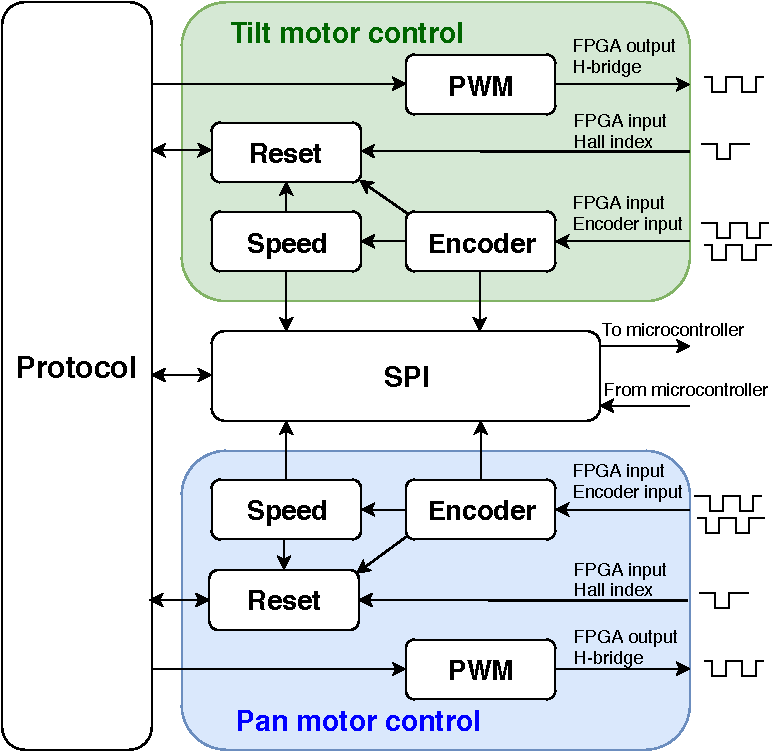
\includegraphics[width=0.8\textwidth]{Sections/System_Implementation/Images/FPGALogicBothMotors.pdf}
    \caption{Overview of the relation between the implemented modules on the FPGA. Arrows indicate information flowing towards a module. Double arrows indicate information flows both ways between two modules}
    \label{fig:FPGALogicBothMotors}
\end{figure}

\begin{figure}[H]
    \centering
    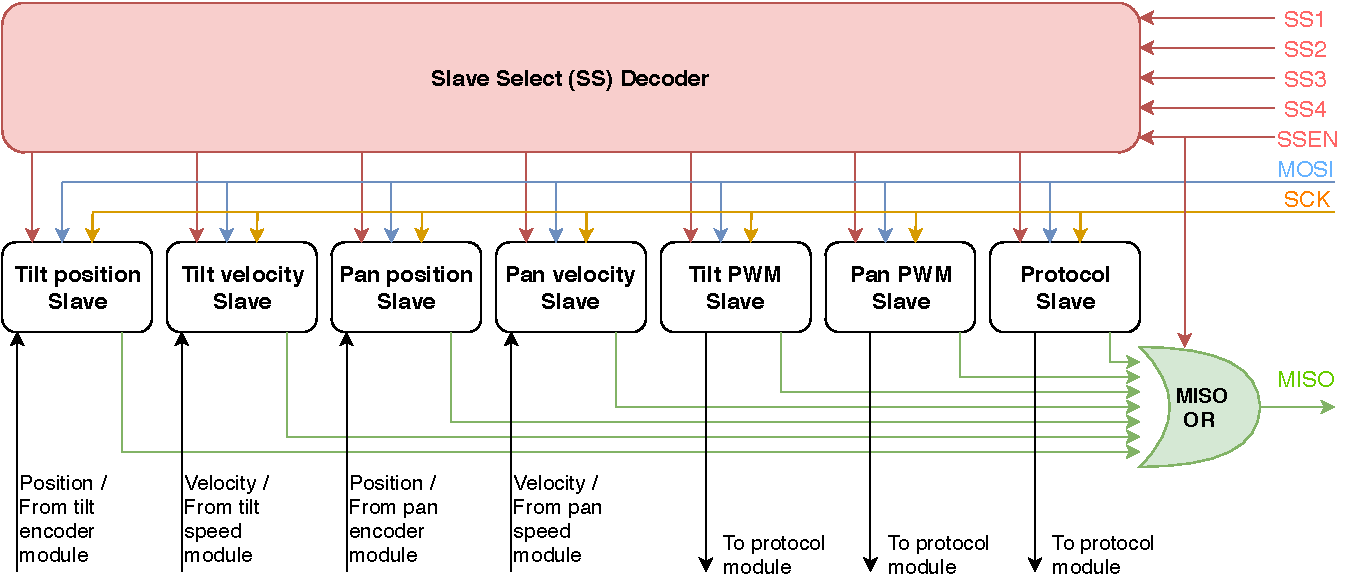
\includegraphics[width=\textwidth]{Sections/System_Implementation/Images/SPILogicSimple.pdf}
    \caption{Overview of the SPI module implemented on the FPGA, showing the seven slaves and the slave-select-module and logical MISO OR-module used to choose between the slaves. All colored signals interface with the microcontroller which is the SPI Master. } % through just one PMOD-connector on the Basys 3 - kit }
    \label{fig:SPILogicSimple}
\end{figure}

\begin{wrapfigure}[25]{R}{0.4\textwidth}
\centering
\caption{Process in FPGA that handles changing the direction if the reset is stuck}
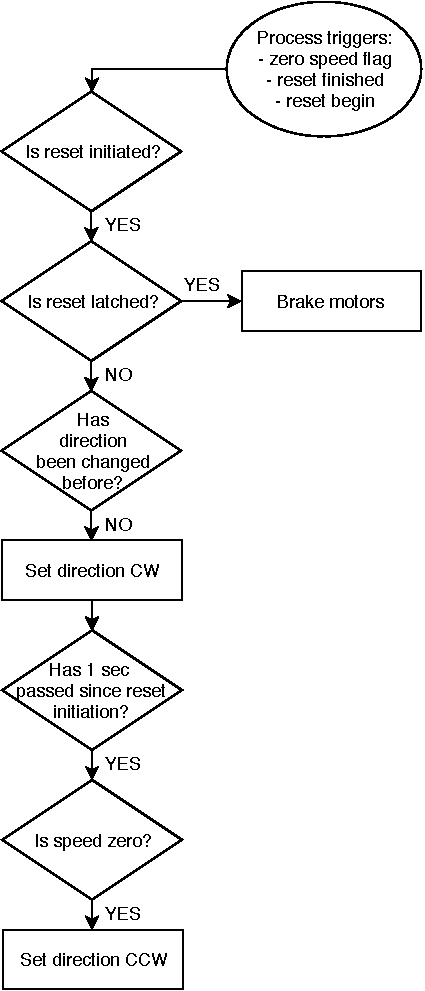
\includegraphics[width = 0.35\textwidth]{Sections/System_Implementation/Images/FPGAFlowchartsResetDirection.pdf}
\label{fig:FPGAFlowchartsResetDirection}
\end{wrapfigure}

\subsubsection*{Encoder Logic}

Each motor is equipped with an Encoder module. The Encoder module is a quadrature incremental encoder with 360 pulses for one revolution of the motor shaft. The encoder provides information via its two outputs channel A and channel B, from where a direction and a position relative to the previous position can be calculated. An index is provided, so a fixed reference is given for initialising the position measurement. The Encoder module looks at channel A and B continuously and enables a count whenever a falling or rising edge occur on either of the channels. The angular velocity is calculated based on the assumption that change in position of the output shaft per encoder count is equal. Later this assumption was discovered to be wrong, the consequences will be discussed in section \ref{sec:Discussion}.


% The distance between rising edges or falling edges of the same channel is the same, though still relative to the speed. However in between the falling edge and rising edge of one of the channels there must be an edge in either direction from the other channel and it is not guaranteed that this edge occurs with the same distance to the aforementioned rising and falling edge.  




\subsubsection*{Reset Logic}
The controllers needs a reference point to initialise position measurement.
The Reset module is responsible for resetting the pan or tilt frame to its index position. When a reset routine is enabled from the Protocol module, the motors drives the pan-tilt frames with constant low duty cycle until a pulse from the respective index hall sensors are received. If the pan frame is stopped during a reset, due to physical limitations in the setup, the frame reverts the direction of rotation. When it receives the pulse the Reset module brakes the motors while pulsing the Encoder module to reset its encoder value to 0. Figure 


 Figure \ref{fig:FPGAFlowchartsResetLatchAndIndex} shows the flow in the process that receives the pulse from the index hall sensor. When it receives the pulse the module immediately brakes the motors while pulsing the Encoder module to reset its encoder value to 0. 
 The Reset module has logic to drive the motors in the opposite direction when the speed of the motors has been zero for a set time-period as is necessary for the pan frame. Figure \ref{fig:FPGAFlowchartsResetDirection} shows a flowchart of the logic that is responsible for changing the direction. 





%

\subsubsection*{Speed Logic}
The Speed module calculates a speed given by the time period between two encoder ticks. As the Speed module is provided with a clock of \SI{100}{\kilo \hertz}, the units for the FPGA output speed is described by $\left[\dot{\theta}_{FPGA}\right] = \frac{\SI{10}{\micro \second}}{\mathrm{tick_{enc}}}$, where $\mathrm{tick_{enc}}$ is the encoder ticks. However a conversion is made in the microcontroller to convert the result to have the units \[ \left[ \dot{\theta}_m \right] = \SI{}{\radian \per \second } \] with respect to the motor. The motor encoder on the motor has 360 encoder ticks per revolution, which means that the relation between the angle of the motor measured in radians and the encoder ticks is, $\pi / 180$. As a result the conversion that is made microcontroller is given by equation \ref{eq:velocity_motor}.
\begin{equation}\label{eq:velocity_motor}
    \dot{\theta}_{m} = \frac{\frac{\pi}{180}}{ \dot{\theta}_{\mathrm{FPGA}} }\cdot 10^{5}
\end{equation}

The Speed module is also responsible for setting and clearing a flag, which indicates whether the speed is zero or not. A change in encoder position must happen within a set time period for the flag to be cleared. In figure \ref{fig:FPGAProcessSpeedFlowcharts} a flowchart of the logic in the module is provided.

\begin{figure}[h]
\begin{subfigure}{0.48\textwidth}
    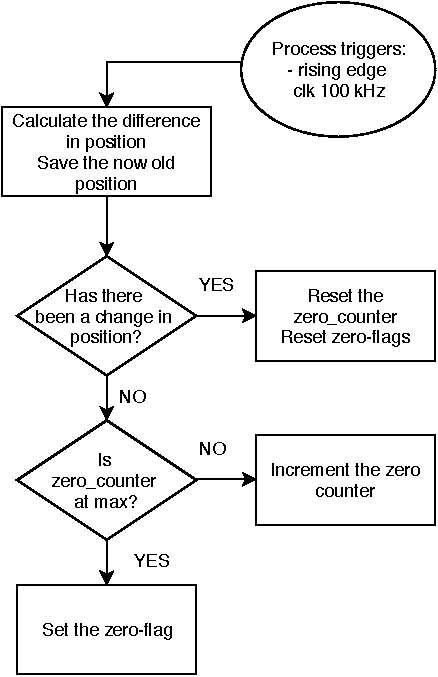
\includegraphics[width = 0.97\textwidth]{Sections/System_Implementation/Images/FPGAProcessSpeedZeroFlowchart.pdf}
    \caption{Flowchart of the process that sets or clears the zero flag}
    \label{subfig:FPGAProcessSpeedZeroFlowchart}
\end{subfigure}\quad
\begin{subfigure}{0.48\textwidth}
    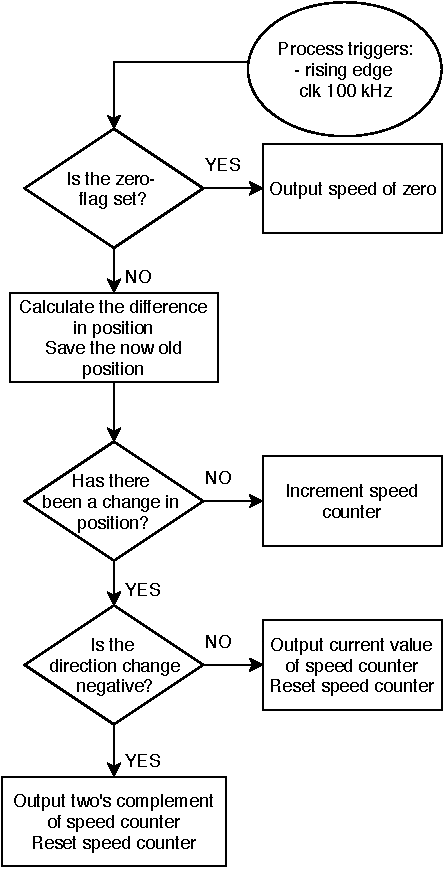
\includegraphics[width = 0.97\textwidth]{Sections/System_Implementation/Images/FPGAProcessSpeedOutputFlowchart.pdf}
    \caption{Flowchart of the process that outputs the speed}
    \label{subfig:FPGAProcessSpeedZeroFlowchart}
\end{subfigure}
\caption{Flowcharts of the logic in the Speed module}
\label{fig:FPGAProcessSpeedFlowcharts}
\end{figure}



\subsubsection*{Protocol decoder logic}


The protocol decoder module is designed as seen in figure (\ref{fig:ProtocolDecoderLogic}). It determines which modules has access to the PWM module and thus controlling the robot. The two modules that need access are the Reset module and the SPI module. As default the SPI module controls the PWM and direction of the robot. As seen on figure \ref{fig:SPILogicSimple}, a separate SPI slave is connected to the protocol module which allows for the microcontroller to transmit a signal telling the reset module, when to control the PWM and the direction of the motors. When the signal is received the SPI cannot change anything regarding the PWM or direction until the reset is completed. 

%\clearpage


\begin{wrapfigure}[24]{R}{0.4\textwidth}
\centering
    \caption{process in FPGA that handles latching a reset and sending a signal to reset the encoder-module}
    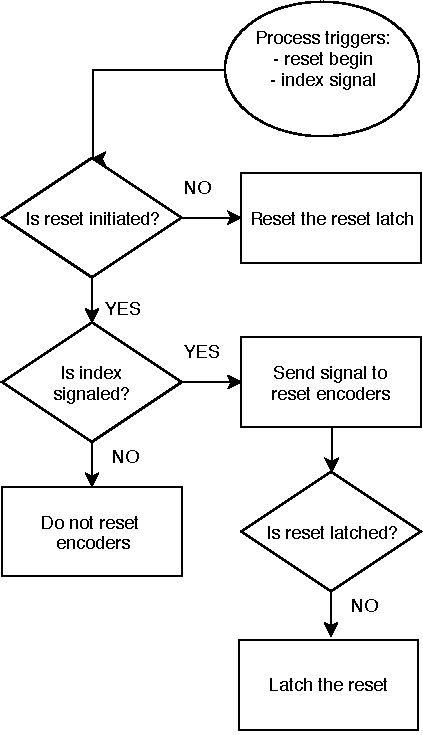
\includegraphics[width=0.35\textwidth]{Sections/System_Implementation/Images/FPGAFlowchartsResetLatchAndIndex.pdf}
    \label{fig:FPGAFlowchartsResetLatchAndIndex}
\end{wrapfigure}

\subsubsection*{SPI Logic}




On figure \ref{fig:SPILogicSimple} an overview of the SPI module is shown. It contains seven internal slaves where four of them hold information needed by the microcontroller, two hold the PWM and directed from the microcontroller that is needed to control the motors and the last slave is used to give certain messages to the FPGA to initialise different states. When a specific kind of data is needed, the microcontroller set the slave select, SS, according to the slave number, low and the decoder activates the slave requested. When transmitting data only one slave can be active at any time and as default the output of a slave is low witch enables that active slave to take over MISO when OR'ed together with the other slaves. The Slave Select Enable, SSEN, is controlled by the hardware of the microcontroller and is used as an enable pin for the SPI. The values of the internal slaves is constantly updated and always contains the newest data, but when the data needs to be transmitted a latch is used to avoid the data changing while transmitting. 
When data is transmitted to the FPGA the same method is used. Rhe decoder activates a specific slave and only the active slave can access the data on MOSI. The data received is first available to other modules on the FPGA when the transmission is complete. 

\begin{figure}[h]
\begin{subfigure}{0.48\textwidth}
    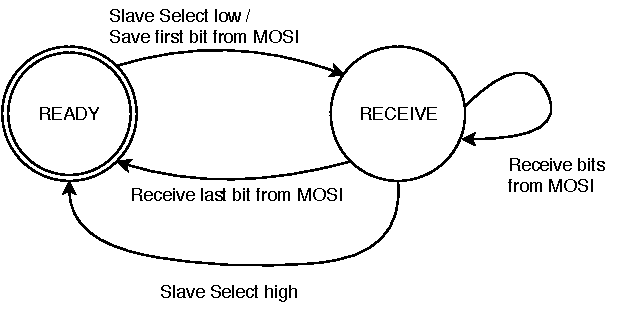
\includegraphics[width = 0.97\textwidth]{Sections/System_Implementation/Images/FPGAStateDiagramReceiveSPI.pdf}
    \caption{SPI receive state diagram}
    \label{subfig:FPGAStateDiagramReceiveSPI}
\end{subfigure}\quad
\begin{subfigure}{0.48\textwidth}
    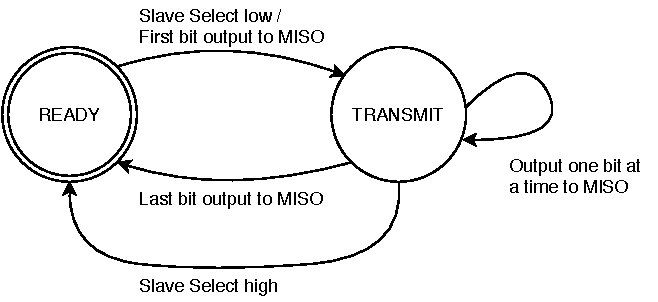
\includegraphics[width = 0.97\textwidth]{Sections/System_Implementation/Images/FPGAStateDiagramTransmitSPI.pdf}
    \caption{SPI transmit state diagram}
    \label{subfig:FPGAStateDiagramTransmitSPI}
\end{subfigure}
\caption{State diagrams for the SPI-module on the FPGA}
\label{fig:FPGAStateDiagramsSPI}
\end{figure}

\clearpage

Figure \ref{ig:FPGAStateDiagramsSPI} illustrates the implementation of SPI on the FPGA. A SPI slave is activated when the associated slave select goes low. Using the clock received from the master, the SPI slave is notified when to transmit and ready data on MOSI. This is done simultaneously utilising the multitasking abilities of the FPGA. Two events can trigger the Slave to change state to ready again, either the slave is done transmitting and receiving or the slave select goes high again. When this happens the module resets and is ready to be used when triggered.

\begin{figure}[]
    \centering
    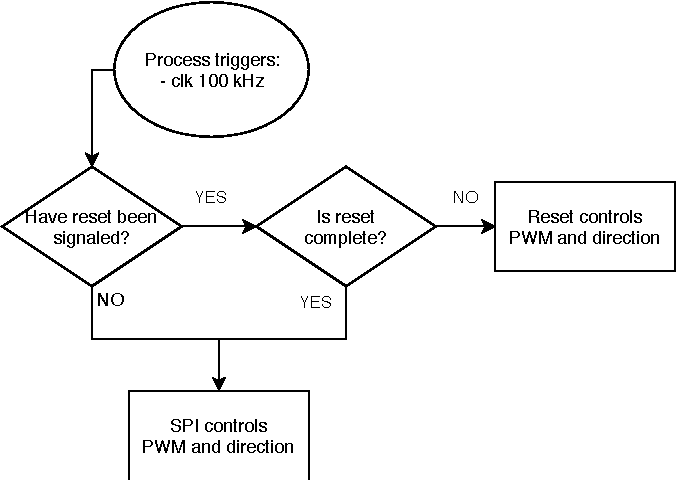
\includegraphics[width=0.5\textwidth]{Sections/System_Implementation/Images/FPGAflowcharts-protocol.pdf}
    \caption{Flowchart of the logic in the Protocol decoder module}
    \label{fig:ProtocolDecoderLogic}
\end{figure}

\end{document}